\documentclass{article}

\usepackage{amsmath, amssymb}
\usepackage{physics}
\usepackage{french}
\usepackage[margin=2.5cm]{geometry}
\usepackage{graphicx}

\begin{document}

\title{Devoir 3 : Équation de Schrödinger en dimension 1} 
\author{PHQ404} 
\date{Remise : 23 mars 2022 à 23h59}
\maketitle

\section{Objectif}

L’objectif de ce TP est de se familiariser avec deux techniques pour solutionner des problèmes aux limites
en dimension 1 : la méthode du tir et la méthode des éléments finis.
Ces méthodes sont présentées au chapitre 12 des notes de David Sénéchal.

\section{Comment présenter et remettre votre TP}

Vous devez créer un dépôt Git pour votre devoir.
Dans ce dépôt, on doit retrouver le code permettant de réaliser le devoir 
ainsi qu'un court rapport. 
Le nom de votre dépot doit être \textit{devoir3\_personne1\_personne2}.
Pour le code, vous devez utiliser Poetry pour gérer votre environnement virtuel.

De plus, le fichier README de votre projet doit indiquer comment obtenir le rapport.
Celui-ci peut-être effectué en \LaTeX\ ou à l'aide d'un carnet numérique (Jupyter ou autre).
Si vous utilisez un carnet, celui-ci ne doit contenir que le code nécessaire pour votre rapport.
Les implémentations doivent se trouver dans un module que vous importez.
Si vous utilisez \LaTeX, il n'est pas nécessaire de soumettre le rapport compilé.
Il est suffisant d'indiquer quel fichier compiler pour obtenir le rapport.

Sauf indication contraire de votre part, 
la dernière version de votre dépôt avant la remise sera évaluée.

\section{Énoncé}

\subsection{Méthode du tir} 

On considère l’équation de Schrödinger indépendante du temps pour une particule de masse unité dans
un potentiel quadratique
\begin{equation}
    - \frac{1}{2} \ddot{\psi} + \frac{1}{2} x^2 \psi = E \psi.
    \label{eq:schrodinger}
\end{equation}
On cherche les solutions pour $x$ de $-L$ à $L$ pour $L = 5$ avec 200 points 
avec les valeurs initiales $\psi(-L) = 0$
et $\psi(-L) = 0.001$. Vous devez :\begin{equation}
    - \frac{1}{2} \ddot{\psi} + \frac{1}{2} x^2 \psi = E \psi.
    \label{eq:schrodinger}
\end{equation}
On cherche les solutions pour $x$ de $-L$ à $L$ pour $L = 5$ avec 200 points 
avec les valeurs initiales $\psi(-L) = 0$ et $\dot \psi(-L) = 0.001$.
La valeur initiale de $\dot \psi$ n'est pas très importante, 
mais celle-ci devrait vous donnez une échelle raisonnable. Vous devez :
\begin{itemize}
    \item 
    Implémenter une fonction qui évalue $\psi(x = L|E)$ comme définie dans les notes.
   
    \item 
    Implémenter une fonction pour cadrer une racine. 
    C’est-à-dire, une fonction qui à partir d’une valeur $x_0$ et d’une fonction $f$,
    trouve une valeur $x_1$ telle que $f(x_1) = -f(x_0)$.
    Pour ce faire, on augmente $x$ par pas de $\Delta$ jusqu’à trouver 
    $x_1$ ou atteindre un nombre limite de pas (20 par exemple).
   
    \item 
    Trouver les racines de $\psi(x = L|E)$ à l’aide de l’algorithme de Brent et de la fonction précédente.

    \item 
    À l’aide de ces fonctions, écrivez un programme qui trouve les 6 premières solutions à l’équation de
    Schrödinger (les 6 énergies les plus basses) et portez-les sur un même graphique en les décalant par la
    valeur de leur énergie, comme illustré à la figure \ref{fig:exemple}.
\end{itemize}

\begin{figure}
    \centering
    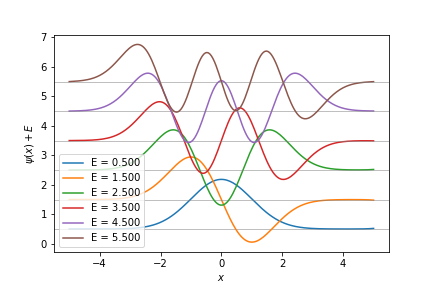
\includegraphics[scale=0.5]{exemple.png}
    \caption{Exemple de figure pour les états propres de basses énergies 
    de l'équation \ref{eq:schrodinger}.}
    \label{fig:exemple}
\end{figure}

\subsection{Méthode des éléments finis}

Dans cette partie, la méthode des éléments finis sera utilisée. 
La méthode n’a pas besoin d’être programmée entièrement~:~un fichier python est fourni 
et doit être importé dans votre programme. 
Ce fichier introduit une classe pour vous aider.
Appliquez la méthode des éléments finis à la solution de la même équation qu’à la partie précédente. 
Cette fois, utilisez une grille de 500 points et une borne $L = 6$. 
Produisez le même type de graphique.
Idéalement, vous utiliseriez la même fonction pour le graphique que pour l'énoncé précédent.
Les fonctions de la classe ne calculent pas les valeurs aux frontières. 
Celles-ci ne sont nécessaire et peuvent ajouter du bruit à vos solutions.

\section{Information complémentaire}

Dans ce devoir, il n'est pas explicitement demandé de vérifier vos solutions 
puisque vous pouvez simplement valider si vous obtenez le bon graphique. 
Par contre, nous vous encourageons tout de même à vérifier les étapes intermédiaires 
de votre code lors de l'implémentation. 

De plus, il est tout à fait raisonnable d'utiliser la bibliothèque scipy pour 
résoudre des intégrations, appliquer la méthode de Brent et résoudre des équations
aux valeurs propres.

\section{Critères d'évaluation}

\begin{description}
  \item[50 points] Pour la méthode du tir.
  \item[40 points] Pour la méthode des éléments finis.
  \item[10 points] Pour la qualité générale du rapport.
\end{description}

\end{document}
